\documentclass[12pt]{article}
\usepackage{hyperref}

\usepackage{graphicx}
\usepackage{color}
\usepackage{fancyvrb}
\usepackage{pastie}

\usepackage{amsthm, amsmath, amssymb, amsfonts, mathrsfs}

\renewcommand{\topfraction}{0.85}
\renewcommand{\textfraction}{0.1}



%%%%%%%%%%%%%%%%%%%%%%%%%%%%%%%%%%%%%%%%%%%%%%%%%%%%%%%%%%%%%%%%%%%%%%%%
\usepackage{color}
\newcommand{\doublecheck}[1]{#1}
\renewcommand{\doublecheck}[1]{\colorbox{yellow}{#1}}

\newcommand{\cc}{\colon\thinspace}

\newcommand{\scA}{\mathcal{A}}
\newcommand{\scB}{\mathcal{B}}
\newcommand{\scC}{\mathcal{C}}
\newcommand{\scE}{\mathcal{E}}
\newcommand{\scF}{\mathcal{F}}
\newcommand{\scG}{\mathcal{G}}
\newcommand{\scO}{\mathcal{O}}
\newcommand{\scX}{\mathcal{X}}
\newcommand{\scY}{\mathcal{Y}}

\newcommand{\bfd}{\mathbf{d}}
\newcommand{\bfr}{\mathbf{r}}
\newcommand{\bfS}{\mathbf{S}}
\newcommand{\bfx}{\mathbf{x}}
\newcommand{\bfy}{\mathbf{y}}
\newcommand{\1}{\mathbf{1}}
\newcommand{\0}{\mathbf{0}}

\newcommand{\bbQ}{\mathbb{Q}}
\newcommand{\bbR}{\mathbb{R}}
\newcommand{\bbZ}{\mathbb{Z}}

\newcommand{\Ot}{\tilde{O}}
\newcommand{\Tt}{\tilde{\Theta}}
\newcommand{\Mt}{\tilde{\Omega}}

\newcommand{\given}{\;|\;}
\newcommand{\biggiven}{\;\big|\;}
\newcommand{\bigggiven}{\;\bigg|\;}

\newcommand{\poly}{\operatorname{poly}}
\newcommand{\Bi}{\operatorname{B}}
\newcommand{\area}{\operatorname{area}}
\renewcommand{\Pr}{\mathbf{P}}
\newcommand{\E}{\mathbf{E}}
\newcommand{\RMSE}{\operatorname{RMSE}}
\newcommand{\dens}{\mathbf{p}}
\renewcommand{\d}{\mathbf{d}}
\newcommand{\logit}{\operatorname{logit}}
\newcommand{\probit}{\operatorname{probit}}

\newcommand{\GammaDist}{\operatorname{Gamma}}
\newcommand{\Poisson}{\operatorname{Poisson}}
\newcommand{\Beta}{\operatorname{Beta}}
\newcommand{\Normal}{\operatorname{Normal}}
\newcommand{\MVNormal}{\operatorname{MVNormal}}
\newcommand{\NegativeBinomial}{\operatorname{NegativeBinomial}}
\newcommand{\Uniform}{\operatorname{Uniform}}
\newcommand{\NBRate}{\operatorname{NBRate}}
\newcommand{\Matern}{\operatorname{Matern}}
\newcommand{\GP}{\operatorname{GP}}
\newcommand{\clip}{\operatorname{clip}}

\newcommand{\true}{\text{true}}
\newcommand{\sex}{\text{sex}}
\renewcommand{\year}{\text{year}}
\newcommand{\regions}{\text{regions}}
\newcommand{\median}{\text{median}}
\newcommand{\CSMR}{\text{CSMR}}
\newcommand{\with}{\text{with}}
\newcommand{\all}{\text{all}}

\def\calC{\mathcal{C}}
\def\calD{\mathcal{D}}

\def\boldpi{{\boldsymbol{\pi}}}
\def\boldw{{\mathbf{w}}}
\def\boldmu{\boldsymbol{\mu}}
\def\boldgamma{\boldsymbol{\gamma}}

\def\PLGP{\operatorname{PLGP}}
\def\PCGP{\operatorname{PCGP}}

\def\a{\alpha}
\def\b{\beta}
%\def\d{\delta}
\def\D{\Delta}
\def\e{\epsilon}
\def\f{\phi}
\def\g{\gamma}
\def\G{\Gamma}
\def\k{\kappa}
\def\la{\lambda}
\def\K{\Kappa}
\def\z{\zeta}
\def\th{\theta}
\def\Th{\Theta}
\def\l{\lambda}
%\def\L{\Lambda}
\def\m{\mu}
\def\n{\nu}
\def\p{\pi}
\def\P{\Pi}
\def\r{\rho}
\def\R{\Rho}
\def\s{\sigma}
\def\S{\Sigma}
\def\t{\tau}
\def\om{\omega}
\def\Om{\Omega}

\newcommand{\proofstart}{{\bf Proof\hspace{2em}}}
\newcommand{\proofend}{\hspace*{\fill}\mbox{$\Box$}}



\begin{document}

\section{Key Equations}

Estimating equation prevalence with random and fixed effects:
\begin{align*}
\dens(p_i\given \pi_i, \delta_i, n_i) &\propto
 \frac{\Gamma(\lfloor p_in_i \rfloor+\delta_i)}{\Gamma(\delta_i)}
 \left(\frac{\delta_i}{\pi_i+\delta_i}\right)^\delta_i \left(\frac{\pi_i}{\pi_i+\delta_i}\right)^{\lfloor p_in_i\rfloor}\\
\pi_i &= \int_{a={a_s}_i}^{{a_e}_i} \boldpi(a) e^{\alpha U_i + \beta X_i + \beta' X'_i} \d w_i(a)\\
\alpha_j &\sim \Normal\left(0, \sigma_{\ell(j)}^2\right)\\
\delta_i &= e^{\eta + \zeta Z_i}
\end{align*}


I represent a spline model for an age-specific hazard $\boldpi(a)$ by a set
of knots $a_1,\dots,a_{K}$, and a set piecewise polynomial basis
functions $\{p_1,\ldots,p_{K'}\}$.  Each knot has a corresponding
basis function, and for higher order splines, there may be additional
basis functions as well, so $K \leq K'$.  The model then has $K'$
parameters, $\gamma_1,\ldots,\gamma_{K'}$, and takes the form
\[
\boldpi(a) = \sum_{k=0}^{K} \gamma_k p_k(a),
\]
or
\[
\boldpi(a) = \gamma_0 + \sum_{k=1}^K \gamma_k a \1[a \geq a_k],
\]
where
\[
\1[a \geq a_k]
=
\begin{cases}
1,&\quad\text{if } a \geq a_k;\\
0,&\quad\text{otherwise;}
\end{cases}
\]
and $\gamma_k$ are the age fixed effect parameters.



By taking the piecewise polynomial corresponding to each knot as zero
before its knot and a linearly increasing function after, the model
specializes to a piecewise constant spline model, a continuous
function that has a constant derivative at all non-knots.  By adding
an additional basis function that is not associated with a knot, this
piecewise linear spline model becomes a flexible approximation for any
nonlinear function, and is the main form I have used in representing
age-specific hazards in the work to come.  I can write out the
piecewise constant specialization of the spline model as
\[
\boldpi(a) = \gamma_0 + \sum_{k=1}^K \gamma_k a \1[a \geq a_k],
\]

I find that in applications of this model it is useful to represent
the piecewise linear spline in an alternative basis, where the model
parameter $\gamma_k$ represents the values of $h(a_k)$ instead of the
change in the slope at this point.  This yields a more complicated set
of basis functions, but it is not necessary to write out the basis
functions explicitly.






Smoothing is accomplished by:

\[
\left(\int _{a=a_1} ^{a_K} \left\| \frac{d \log \boldpi (a)}{da} \right\|^2 dw(a)\right)^{1/2} \sim N(0, \sigma^2).
\]


Increasing prior:

\[
\operatorname{clip}(\log \boldpi(a+1) - \log \boldpi(a), 0, 1) \sim \Normal(0, \epsilon^2),
\]
for a small value of $\epsilon$, like $\epsilon = 10^{-6}$.


\section{Introduction}
The estimation of years lived with disability (YLDs) from sparse,
noisy data is quite a technical challenge.  We used a model-based
meta-analytic method for descriptive epidemiology that was developed
specifically to meet this challenge.  This approach is based on an
integrative systems model for disease in populations, and relies on
Bayesian methods to estimate the model parameters from the sparse,
noisy data available.  This builds on work in generic disease modeling
that has been in use for almost twenty years in global health
epidemiology \cite{Barendregt_Generic_2003}, and has recently been
collected together in book form.

The integrative systems modeling approach formally connects a system
dynamics model of disease progression to a statistical model of
epidemiological rates.  The system dynamics model is a ``model of
process'', describing how disease progresses through a population by a
compartmental model and corresponding system of differential
equations.  The statistical model is a ``model of data'', which is a
random-effects generalized negative binomial, augmented by an
age-standardization approach to deal with the overlapping
heterogeneous age groups found in systematic review.

Parameter estimation in this model was achieved by Bayesian methods,
using a combination of derivative-free optimization and Markov chain
Monte Carlo.  The model is fit with an empirical Bayes approach, in
two stages.  First, we produced a global estimate by pooling data
globally.  Then the regional predictions were used as empirical priors
to produce region/sex/year-specific estimates together with only the
data relevant to each region/sex/year.

This appendix describes the model of process, the model of data, and
the numerical algorithms in detail.  Section~\ref{process} develops
the model of process, which consists of a compartmental model of
disease in a population, a spline model for the key parameters of the
compartmental model (incidence, remission, and excess-mortality) as
functions of age, and expert priors on the structure of the age
pattern.  Section~\ref{data} addresses the model of data, which links
the model of process to the data collected in systematic review.  This
rests on a negative binomial model for epidemiological rates, which is
augmented with fixed and random effects to explain heterogeneity based
on explanatory variables and unexplained spatial variation.  It also
includes an age-standardization approach to deal with the
heterogeneous age groups found in systematic review.  Section~\ref{na}
describes the computational methods used to fit the integrative
systems model, an empirical Bayesian approach which relys on the
Markov chain Monte Carlo algorithm.

\section{Model of process}
\label{process}
Integrative systems modeling (ISM) combines system dynamics modeling
with statistical modeling, by using a ``mechanistic'' model of process
together with a statistical model of data.  The foundations of ISM are
best articulated in terms of \emph{system dynamics modeling}, a
discipline that originated in the fields of operations research and
industrial engineering \cite{Forrester 1961. Industrial
  dynamics. Waltham, MA: Pegasus Communications} \cite{Forrester
  1969. Urban Dynamics. Pegasus Communications} \cite{Forrester
  1971. World Dynamics. Wright-Allen Press} \cite{Forrester
  1971. World Dynamics. Wright-Allen Press}
\cite{Meadows_Thinking_2008}.

System dynamics modeling is a method to model the behavior of complex
systems in terms of stocks, flows, and feedback loops.  In short,
\emph{stock variables} quantify the amount of some material, or mass,
or population in a compartment at a particular moment in time, while
\emph{flow variables} quantify the rate of material moving into, out
of, or between compartments.


\subsection{Compartmental model}
The progress of a disease through a population can be represented
generically by a two-compartment system dynamics model of process,
which represents the ``fundamental equations'' of population
health. The compartments contain the population susceptible to the
disease (stock $S$, for ``susceptible'') and the population with the
condition (stock $C$, for ``condition''). The population moves between
these compartments following the arrows shown in
Figure~\ref{forward-sim-two-compartment}, transitioning from $S$ to
$C$ with incidence rate $i$, and from $C$ back to $S$ with remission
rate $r$. The susceptible population flows out of the system with
background mortality rate $m$, and the with-condition population flows
out of the system with with-condition mortality rate $m+f$.  Here $f$
represents the ``excess mortality rate'' for individuals with the
condition over individuals without the condition.

\begin{figure}[h]
\begin{center}
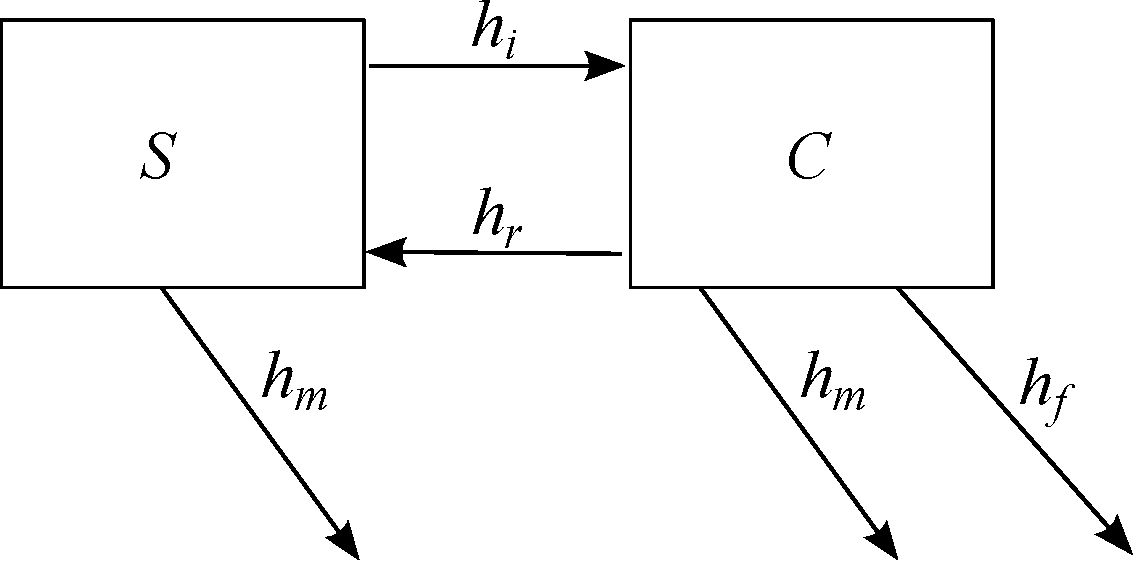
\includegraphics[width=3in]{SC.pdf}
\caption{The two-compartment model of process for disease in a
  population, around which the meta-regression framework is
  built. Compartment $S$ contains the population susceptible to the
  disease and compartment $C$ contains the population with the
  condition. Individuals move from $S$ to $C$ with incidence rate $i$,
  and from $C$ to $S$ with remission rate $r$. The susceptible
  population flows out of the system with without-condition mortality
  rate $m$, and the with-condition population flows out of the system
  with with-condition mortality rate $m+f$, where $f$ is the excess
  mortality rate, representing quantitatively the increase in
  mortality for individuals with the condition.}
\label{forward-sim-two-compartment}
\end{center}
\end{figure}

The schematic depiction of the system dyanmics model in
Figure~\ref{forward-sim-two-compartment} is made precise by a system
of partial differential equations, which correspond to the stocks and
flows above, and more precisely represent their relationship as a
function of time and age:
\begin{align*}
\frac{\partial S}{\partial (a+t)} &= -(i + m)S + rC,\\
\frac{\partial C}{\partial (a+t)} &= iS - (r + m + f)C,\\
\end{align*}
where
\begin{align*}
S &= S(a,t) = \text{stock of ``susceptibles''},\\
C &= C(a,t) = \text{stock of ``with condition''},\\[.1in]
i &= i(a,t) = \text{incidence rate for susceptibles},\\
r &= r(a,t) = \text{remission rate for individuals with condition},\\
m &= m(a,t) = \text{without-condition mortality rate for any individuals},\\
f &= f(a,t) = \text{excess-mortality rate for individuals with
condition}.
\end{align*}
Here all of these quantities are functions of both age $a$ and time
$t$.

All of the other epidemiological parameters of interest can be derived from these stocks and flows:
\begin{align*}
p &= \frac{C(a,t)}{S(a,t)+C(a,t)} = \text{prevalence},\\
RR &= \frac{m(a,t)+f(a,t)}{m(a,t)} = \text{relative risk},\\
SMR &= \frac{m(a,t)+f(a,t)}{m(a,t)+p(a,t)f(a,t)} = \text{standardized mortality ratio},\\
m_\with &= m(a,t)+f(a,t) = \text{with-condition mortality rate},\\
X &= \int_{\tau = 0}^\infty e^{-\left(r(a+\tau, t+\tau) + f(a+\tau, t+\tau) + m(a+\tau, t+\tau)\right) \tau}\d \tau
= \text{duration of disease}.
\end{align*}

The full model above is often more complex than can be supported by
available data, which is usually very sparse and very noisy.  An
important simplification in almost all known cases is the assumption
that the disease parameters are not changing substantially with
respect to time. To be precise, this assumption that the partial
derivative of all stocks and all flows with respect to time is zero:
\[
\frac{\partial S}{\partial t}
=
\frac{\partial C}{\partial t}
=
\frac{\partial i}{\partial t}
=
\frac{\partial r}{\partial t}
=
\frac{\partial m}{\partial t}
=
\frac{\partial f}{\partial t}
=
0.
\]

This simplifies the partial differential equations to ordinary
differential equations, which can be solved iteratively using standard
algorithms.  We will return to this in Section~\ref{na}.

\subsection{Spline model}

The approach we took for modeling age-specific rates draws
on the mathematical theory of spline interpolation, and the
statistical theory of smoothing splines.

\emph{Splines models} or \emph{piecewise polynomials} refer to a
family of models which result from specific definitions of the basis
functions, $h_i$. These models arise by partitioning the age variable $a$
into $k+1$ contiguous intervals at \emph{knot locations} $\xi_1,
\dots, \xi_{k}$. The spline model $f(a)$ is then represented by different
polynomials in each interval.  We use
a piecewise linear model, which takes the form,
\[
f(a) = \sum_{i=0}^m\beta_m h_m(a),
\]
\[
h_0(a) = 1,\; h_1(a) = a,\; h_2(a) = (a-\xi_1)_+,\; \dots,\; h_{k+2}=(a-\xi_k)_+,
\]
where the notation $h_+$ indicates the positive part of $h$. Models
fit using bases of this type are continuous but not differentiable at
the knot locations.

Depending on the data, the ``knots'' can have almost as much influence
on the fit as the choice of basis functions.  For the purpose of
generic disease modeling, knot locations should be chosen \emph{a
  priori} to reflect expert knowledge about the disease of interest
and its behavior as a function of some continuous variable. For
example, in a recent study looking at global trends in mean systolic
blood pressure as a function of age, Danaei \emph{et al} used a cubic
regression spline with knots located at ages 30 and 60 ($\xi_1 = 30$
and $\xi_2=60$) \cite{Danaei_National_2011}. These choices reflect the
expectation, based on literature and prior knowledge, that the
behavior of mean systolic blood pressure as a function of age would be
distinct in these intervals due to a) low blood pressure in young
adults, and b) survivor effects in elderly populations.

We use smoothing splines to reduce the challenge of knot selection.
The smoothing spline can be formulated in a Bayesian framework in
terms of a prior representing the belief that in the absence of
evidence, the age-pattern is not varying.  Mathematically, this takes
the form of a penalty on the root mean square of the derivative of the
age-specific rate $f$:
\[
\left(\int _{a=a_0} ^{a_1} \| f'(a) \|^2 dw(a)\right)^{1/2} \sim N(0, \sigma^2).
\]

For the piecewise linear smoothing splines that will be used most
frequently in the second half of this book, the derivative of $f$ is
constant between knots, so with equal weighting for smoothing at all
ages, the integral above simplifies to the following:
\[
\int _{a=a_0} ^{a_1} \| f'(a) \|^2 = \sum_{i=0} ^K \bigg(\sum_{j=1} ^{k-1} \beta_j\bigg)^2(k_{i+1}-k_i) / (k_K - k_0)
\]
Figure~\ref{smoothing-splines} shows the effect of increasing the
smoothing parameter $\sigma$.

\begin{figure}[h]
\begin{center}
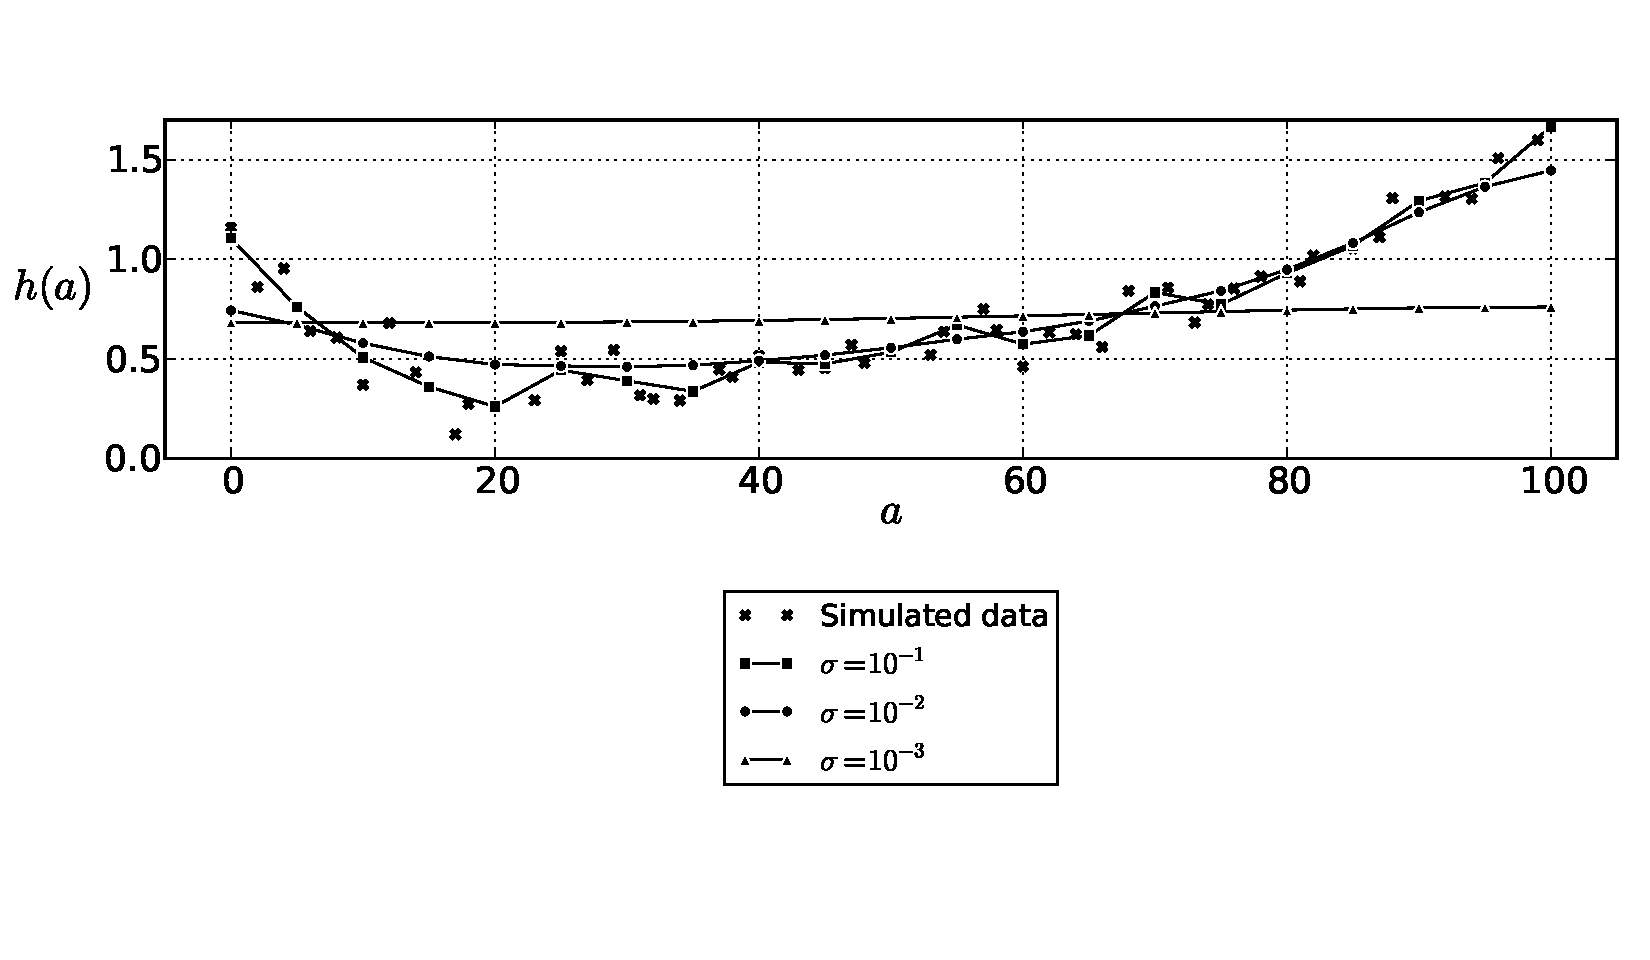
\includegraphics[width=\textwidth]{smoothing-splines.pdf}
\caption{Smoothing splines provide a solution to the challenge of knot
  selection in spline modeling.  Without smoothing, including many
  knots leads to estimates that are overly uncertain and wiggly.
  Smoothing, in the form of a quadratic penalty on the derivative of
  the age pattern, allows many knots to be included.}
\label{smoothing-splines}
\end{center}
\end{figure}

There are a few ways to augment the spline model that are useful when
modeling age-specific rates. Since the rates in the compartmental
model are always non-negative, I have parameterized the spline in
terms of the log of the knot values:
\[
\gamma_i = \log\bigg(\sum_{j=0}^I \beta_i\bigg).
\]
In order to fit the model in a Bayesian framework, I have defaulted to
giving these $\gamma_i$'s ``weakly informative'' priors,
\[
\gamma_i \sim \Normal\left(0, 10^2\right).
\]
This has very little effect on the posterior distribution, but makes
the prior ``proper'' and also helps with algorithm convergence in
some instances. In instances where relevant expert knowledge is
available, I can replace this with a more informative prior (this idea
is elaborated in the following section).

Finally, in order to deal with the order-of-magnitude differences of
age-specific rates, I have applied the spline smoothing to the
log-rate, rather than the rate itself.  This creates an additional
complication, however, because the informative priors often say that
rates are zero for certain ages.  In order to avoid the ill effects of
smoothing when the log-rate contains values of $-\infty$, I have
rounded up any $\gamma_i$ values that are below ten times the mean
rate.


\subsection{Expert priors}
There are three classes of additional information that we bring to
bear on age pattern models, which we collect under the banner of
``expert priors'', because all are implemented in the Bayesian
framework as additional constraints on the prior distribution for the
age pattern models.
\begin{itemize}
\item Level value priors enforce the constraint that the age-specific
rate take a value $v$ on age range $[a_0,a_1]$.  
\item Level bound priors enforce the constraint that the age-specific rate
take values between $\ell_0$ and $\ell_1$.
\item Monotonicity priors enforce the constraint that the age-speicifc
  rate be increasing or decreasing over a certain age range.
\end{itemize}

\section{Model of data}
\label{data}
\subsection{Negative binomial model}
The negative binomial model is an adaptation of the traditional random
effects model in linear regression to the Poisson case, where each
observation comes from a different Poisson model and the Poisson
parameter of these models are all drawn from a common Gamma
distribution. Thus a rate model based on this distribution provides
benefits in handling non-sampling variation.  The negative-binomial
rate model for observing a rate of $r$ from $n$ person-years of observation:
\[
\dens(r\given \pi, \delta, n) \propto
 \frac{\Gamma(\lfloor rn \rfloor+\delta)}{\Gamma(\delta)} (1-\pi)^\delta \pi^{\lfloor rn\rfloor}.
\]

Figure~\ref{rate-model-negative-binomial-funnel} shows funnel plots
for two levels of over-dispersion, as well as the posterior predictive
distribution for the negative binomial model.

\begin{figure}[ht]
\begin{center}
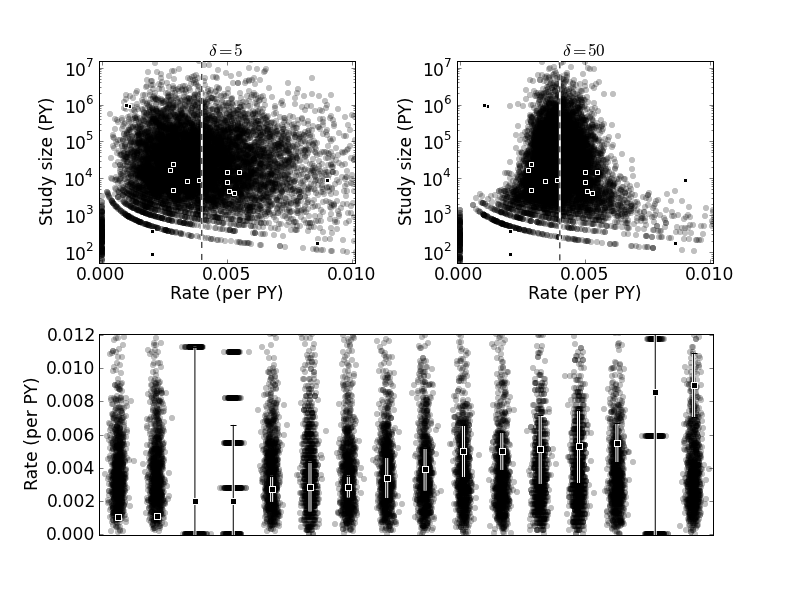
\includegraphics[width=\textwidth]{negative-binomial-funnel.png}

\end{center}
\caption{Funnel plots and posterior predictive check for the negative
  binomial model. This model captures heterogeneity in observed data
  using an ``over-dispersion'' parameter $\delta$, which can be
  interpreted as a hierarchical model, where each observation is drawn
  from a Poisson distribution that has its parameter drawn from a
  Gamma distribution.  When $\delta$ is very large, the negative
  binomial model is equivalent to the Poisson model.  The posterior
  predictive check shows that the uncertainty in the posterior
  predictions contains all of the observed data, indicating that this
  model is sufficiently flexible to represent the observed
  heterogeneity.} \label{rate-model-negative-binomial-funnel}
\end{figure}


\subsection{Covariate model}
In the integrative systems model of disease in populations, covariate
modeling has two distinct goals.  First, covariates are a way to
explain the bias and variation of the noisy measurements of
epidemiological rates.  And second, covariates are a way to increase
the accuracy of out-of-sample predictions.  This is accomplished by
modeling the relationships between the disease parameters of interest
and the explanatory covariates. The modeled relationships are then
used to extrapolate predictions for the disease parameters to
geographic regions where covariate data is available, but no direct
measurements are made.

Let the data collected in systematic review be denoted by tuples
$\left(a_i, n_i, r_i, U_i, X_i\right)$, where $a_i$ is the age group,
$n_i$ is the effective sample size, $r_i$ is the observed rate value,
$U_i$ is an indicator vector of spatial covariates, and $X_i$ is a
vector of explanatory covariate values. The covariate model is then
the following:
\begin{align*}
r_i, n_i &\sim \NBRate\left(\mu_i, \delta\right),\\
\mu_i &= \boldmu(a_i)e^{\alpha U_i+\beta X_i}\\
\alpha_j &\sim \Normal\left(0, \sigma_{\ell(j)}^2\right),
\end{align*}
where $\ell(j)$ is the level in the hierarchy of node $j$, and
$\sigma_\ell$ is also a model parameter. To fit this model with
Bayesian methods, we also need a prior on $\sigma_\ell$ (a
hyper-prior), and because of the sparse and noisy nature of the
available data, this often has to be somewhat informative.  The
truncated normal distribution
\[
\sigma_\ell \sim \Normal_{[.05,5]}\left(.05, .03^2\right),
\]
is often an appropriate choice. It says that between-area variation of
less than 5\% is impossible and more than 15\% is rare.

The parameter $\beta$ represents the effect coefficients for
the fixed effects, and because the data is often sparse and noisy, it
can help the stability of the computational algorithms to put a weakly
informative prior on $\beta$, such as
\[
\beta_j \sim \Normal\left(0, 1^2\right) \text{ for } j = 1, \ldots, J.
\]
Of course, if experts have beliefs about the sign or magnitude of the
effect coefficient, this can be included as a more informative prior.


\subsection{Age-averaging model}
The age groups for data collected in systematic review exhibit extreme
heterogeneity, which makes traditional meta-analysis techniques
impossible.  To address this, we developed a simple mathematical model
of age pooling:
for ages $a_0, a_1, a_2$, the rate for age groups $(a_0,a_1)$, $(a_1, a_2)$ and $(a_0, a_2)$ are related by the equation
\[
r_{a_0,a_2} = \int_{a=a_0}^{a_2} r_{a,a+da}n_{a,a+da}/n_{a_0,a_2}\d a,
\]
where $r_{a,b}$ is the rate for age group $(a,b)$, and $n_{a,b}$ is
the number of person-years of observation for this age group.

To account for this we average across the age interval explicitly in
our statistical model:
\begin{align*}
r_i, n_i &\sim \NBRate\left(\mu_i, \rho\right),\\
\mu_i &= \int_{a=a0_i}^{a1_i} \boldmu(a)\d w(a).
\end{align*}

\begin{figure}[h]
\begin{center}
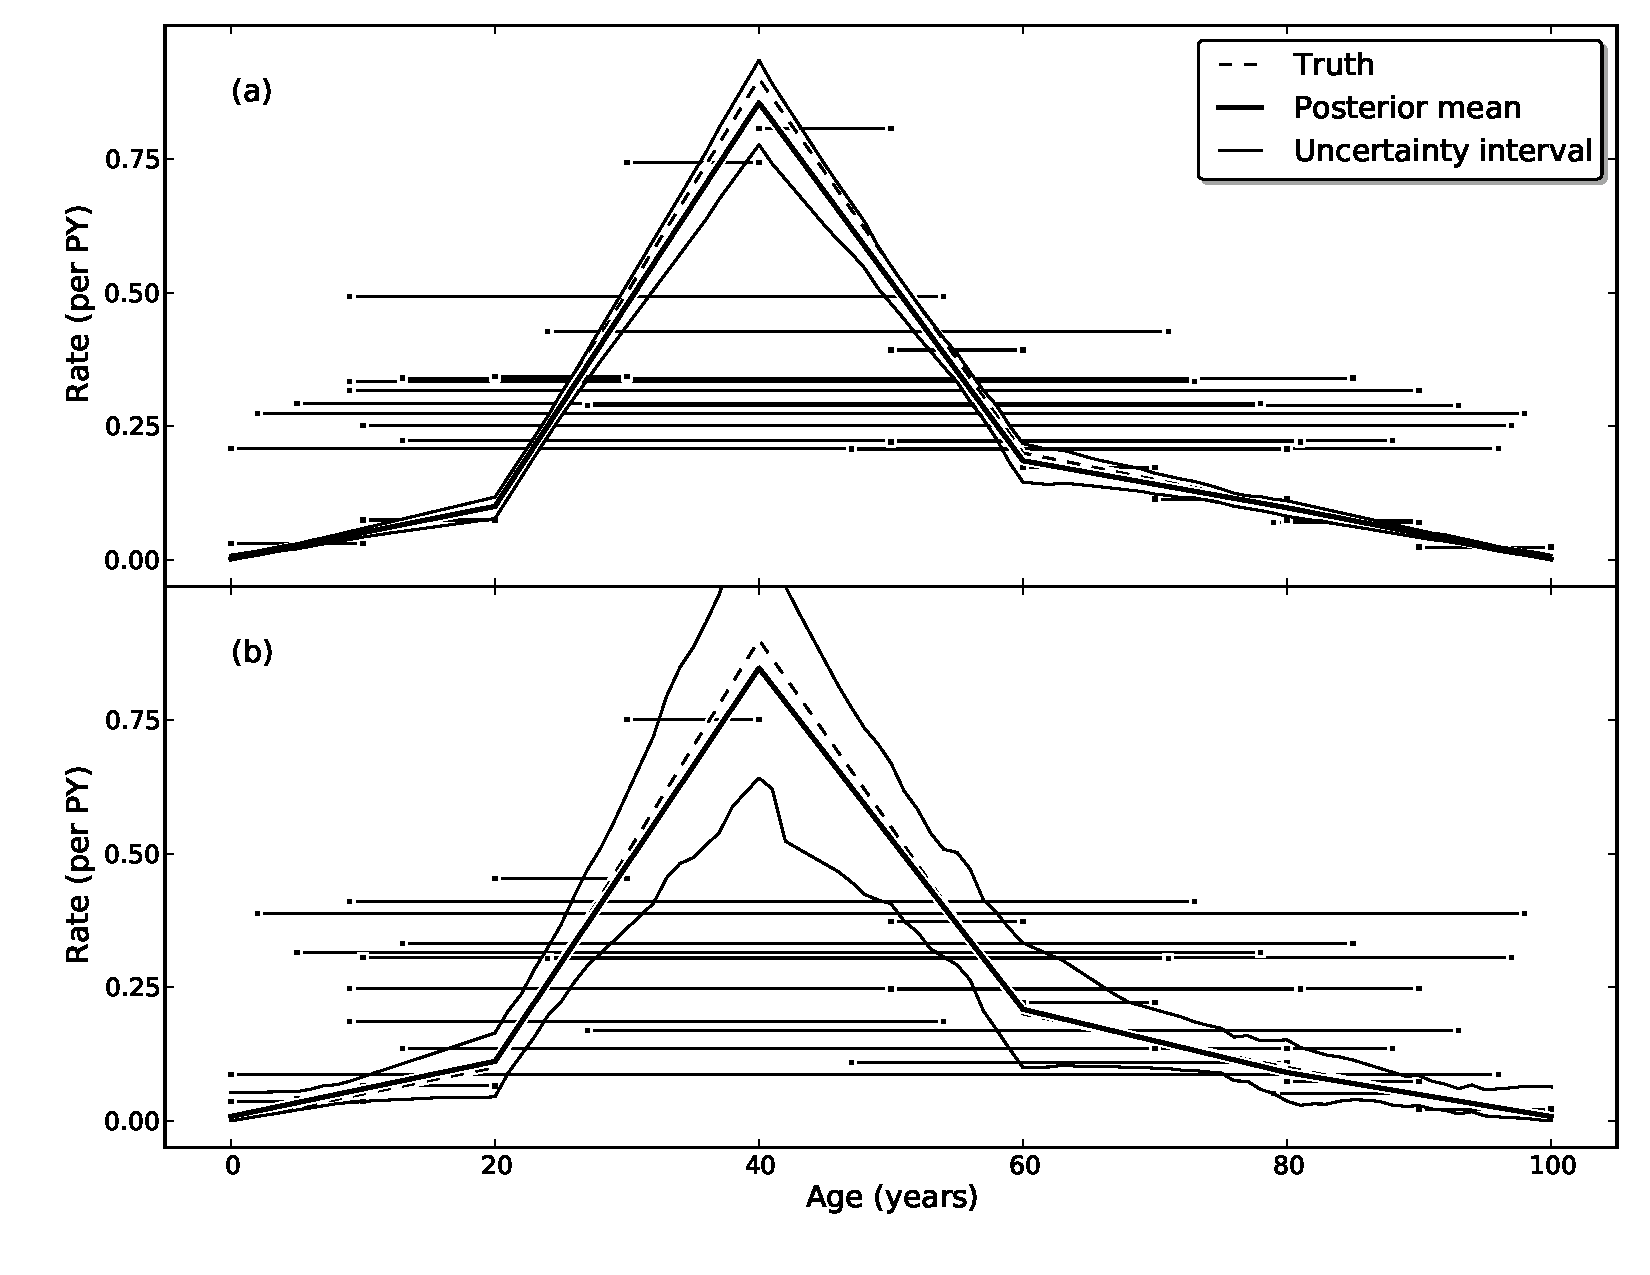
\includegraphics[width=\textwidth]{age_group_standardize.pdf}
\caption{TK caption about Age-standardizing model results in panel (a)
  recover the true age pattern quite precise. Panel (b) shows that the
  results are still accurate when the data generation procedure is
  even more noisy.}
\label{age-group-standardize}
\end{center}
\end{figure}


\section{Numerical algorithms}
\label{na}
This integrative systems model of disease in a population does not
admit a closed form representation for its posterior distribution.
Therefore, we rely on the Markov chain Monte Carlo (MCMC) algorithm to
draw samples of the model parameters from their posterior
distribution.  We use the the Adaptive Metropolis (AM) step method
\cite{Haario_Adaptive_2001}, which provides acceptible performance
without requiring burdensome derivation of customized Gibbs
distributions. To obtain initial values for the MCMC, we use Powell's
method, to optimizes a function of many variables without requiring
derivatives \ref{MJD Powell, An efficient method for finding the
  minimum of a function of several variables without calculating
  derivatives , The Computer Journal (1964) 7 (2): 155-162.  doi:
  10.1093/comjnl/7.2.155}.  To produce estimates that reflect the
heterogeneity of disease patterns globally, but also borrow strength
through partial pooling, we use an empirical Bayes approach to
separate the global model into submodels that can be fit in parallel.

Abstractly, the challenge is the following:


Given
\[
\dens_\text{posterior} \cc \bbR^n\rightarrow \bbR^+,
\]
\[
f \cc \bbR^n \rightarrow \bbR
\]
approximate
\[
\int f(x)\dens_\text{posterior}(x)\d x
\]
quickly and accurately.


To solve the ordinary differential equations of the compartmental
model, we use the Fourth order Runge-Kutta formula \cite{Numerical
  Recipes in Fortran 2nd ed.}.

The empirical bayes approach produces region/sex/year specific
estimates in two stages.  First, all of the data is pooled and fit
with the integrative systems model, to produce globally consistent
estimates of incidence, prevalence, remission, and excess-mortality.
This model is used to produce \emph{inconsistent} estimates of
sex-specific incidence, prevalence, remission, and excess-mortality at
the GBD region level for all years.  In the second stage, the regional
estimates are used as empirical priors on incidence, prevalence,
remission, and excess-mortality, and the fixed and random effect
coefficients are set to their mean first-stage values, and an
integrative systems model is fit for each region/sex/year by keeping
only the relevant data for this region, sex, and time period.

\bibliographystyle{plain}
\bibliography{my_library}
\end{document}
